\chapter{Systemdesign und Implementierung}
Nachdem die benötigten Informationen für die Umsetzung der Applikation erarbeitet wurden, konnte eine Implementierung in Hard- und Software erarbeitet werden, welche in diesem Kapitel beschrieben wird. Die Realisierung des Systems erfolgte unter Verwendung der Software-Applikationen \nameref{sw:ltspice}, \nameref{sw:altium}, \nameref{subsub:diamond} mit \nameref{subsub:aldec} und \nameref{sec:xpresso}. Mit diesen Applikationen wurde das System modelliert und Module simuliert.
\section{Systemübersicht}
\begin{figure}[!h]
	\centering
   	\includegraphics[page=1,width=1.0\textwidth, trim= 5mm 5mm 5mm 5mm, clip=true]{images/pcb/new.PDF}%docu
    \caption{Modulübersicht des Systems ohne mechanische und externe Komponenten}
    \label{fig:system}
\end{figure}
In diesem Kapitel wird das erstellte System und dessen Module näher beschrieben. Dabei wird das System in Analog, Digital, Power und mechanische Komponenten untergliedert.
\begin{itemize}
\item Um das System mit Energie zu versorgen wird eine Stromquelle benötigt, welche in \autoref{sec:supply} beschrieben wird. Da das System für die medizinische Anwendung konzipiert ist, wird zudem die Einspeisung des Systems und des \ac{pc}s des Benutzers beschrieben. Diese Beschreibung ist notwendig, da die Spannungsversorgung des Systems auf dem Verhalten der Einspeisung aufbaut.
\item Das Modul Analog beinhaltet dabei den Transmitter, welcher das zu emittierende Signal generiert, sowie den Receiver, welcher aus einen Bandpassfilter, einer \ac{lna} und einer Digitalisierung besteht.
\item Das Modul Digital beinhaltet hingegen die Ansteuerung des Transmitters und des Receivers sowie die Demodulierung und den Datentransfer zwischen dem System und den \ac{pc} des Nutzers.
\item Das Modul Gehäuse wurde aus der Übersicht entfernt, da dieses das gesamte Messsystem beinhaltet und nur die Schnittstellen für die Anbindung des Transducers, des \ac{pc}s sowie der Stromversorgung zur Verfügung stellt. Aus diesem Grund wurde das Gehäuse zwar vorgesehen, jedoch geht dieses in der aktuellen Entwicklungsphase nicht in die Implementierung des Systems ein.
\end{itemize}
Nachfolgend werden die genannten Module mit Spannungsversorgung, Kommunikation, Steuerung / Demodulierung, der Transmitter, der Receiver mit Bandpass sowie das Gehäuse näher betrachtet sowie erklärt. Zudem werden Aussagen über die Auslegung und die Realisierung dieser Module getroffen um den Leser ein besseres Verständnis des Systems und dessen Umsetzung zu geben.
\begin{figure}[h!]
	\centering
	\begin{subfigure}[t]{0.46\textwidth}
    \centering
\begin{annotatedFigure}
	{\includegraphics[page=4,width=1\textwidth, trim= 0mm 0mm 0mm 0mm, clip=true]{images/pcb/Job2.PDF}}
	\annotatedFigureBox{0.074,0.696}{0.6049,0.952}{A}{0.074,0.696}%bl
	\annotatedFigureBox{0.2058,0.2083}{0.3091,0.3109}{B}{0.3091,0.2083}%br
	\annotatedFigureBox{0.4687,0.3625}{0.7468,0.562}{C}{0.7468,0.3625}%br
	\annotatedFigureBox{0.4694,0.092}{0.7465,0.292}{D}{0.7465,0.092}%br
	\annotatedFigureBox{0.8068,0.3508}{0.9092,0.4337}{E}{0.9092,0.3508}%br
	\annotatedFigureBox{0.8068,0.0948}{0.9092,0.1777}{E}{0.9092,0.0948}%br
	\annotatedFigureBox{0.0725,0.0846}{0.2026,0.5097}{F}{0.0725,0.0846}%bl
	\annotatedFigureBox{0.2086,0.0929}{0.2833,0.1409}{G}{0.2833,0.0929}%br
	\annotatedFigureBox{0.2614,0.3189}{0.4451,0.6469}{H}{0.2614,0.6469}%tl
\end{annotatedFigure}
    \caption{Ground Plane und Komponenten auf der Platinenoberseite. (A) Externe Spannung zu 5 V DC, (B) \ac{ldo}s für analoge und digitale Spannungsversorgung, (C) NXP LPC4337, (D) Lattice MachXO2, (E) JTAG Ports, (F) analoge Signalaufbereitung, (G) \ac{adc}, (H) Transmitter mit xDSL Treiber und RF-Transformator}
    \label{fig:system_layout}
    \end{subfigure}%
    \hfil
    \begin{subfigure}[t]{0.46\textwidth}
    \centering
    \begin{annotatedFigure}
	{\includegraphics[page=5,width=1\textwidth, trim= 0mm 0mm 0mm 0mm, clip=true]{images/pcb/Job2.PDF}}
	\annotatedFigureBox{0.5326,0.4688}{0.7145,0.5429}{I}{0.7145,0.4688}%br
	\annotatedFigureBox{0.4951,0.1948}{0.5671,0.2531}{J}{0.5671,0.1948}%br
	\annotatedFigureBox{0.0042,0.53}{0.185,0.9059}{K}{0.185,0.53}%br
	\annotatedFigureBox{0.2667,0.7646}{0.2667,0.7646}{2}{0.2667,0.7646}%br
	\annotatedFigureBox{0.1276,0.1968}{0.1276,0.1968}{3}{0.1276,0.1968}%br
	\annotatedFigureBox{0.5143,0.3248}{0.5143,0.3248}{4}{0.5143,0.3248}%br
	\annotatedFigureBox{0.1833,0.0448}{0.1833,0.0448}{1}{0.1833,0.0448}%br
\end{annotatedFigure}
	\caption{Power Plane und Komponenten auf Platinenunterseite - (I) 12 \ac{mhz} Resonator, (J) 64 \ac{mhz} Oszillator, (K) Steckverbindungen, (1) Schirm-GND auf Power und Ground Plane, (2) 5 V DC und GND, (3) analoge 3,3 V DC und analoger GND, (4) digitale 3,3 V DC und digitaler GND}
    \end{subfigure}
    \caption{Aufteilung der \acs{pcb}}
\end{figure}
\hfill
\section{Spannungsversorgung}\label{sec:supply}
\begin{figure}[!h]
	\centering
   	\includegraphics[page=2,width=1.0\textwidth, trim= 5mm 48mm 5mm 5mm, clip=true]{images/pcb/new.PDF}%docu
    \caption{Modulübersicht des Systems ohne mechanische und externe Komponenten}
    \label{fig:system}
\end{figure}
Damit das System arbeiten kann, benötigt das System elektrische Energie welche typischerweise von Außen zugeführt wird. Da der Fokus dieser Arbeit nicht auf der Energieversorgung der Dopplerinstrumentierung liegt, wurde als Ausgangsbasis ein externes Schaltnetzteil der Firma SL Power Electronics verwendet, welches bei 230 V AC Netzspannung ein 19 V DC Ausgangsspannung mit 3,1 A liefert. Zudem ist das Netzteil GXM60-19A04 nach EN60601 geprüft und somit für medizinische Anwendungen zugelassen. Versionen für den internen Einbau sind dabei im Bereich von 5 bis 56 V DC beziehbar.\cite{slpower}\\
Um elektromagnetische Störungen im System möglichst gering zuhalten, wurden Potentiale anhand der Arbeitsbereiche der elektronischen Komponenten gruppiert und definiert. Dabei ergab sich ein Potential für die 
\begin{itemize}\itemsep0pt
\item digitale Signalverarbeitung mit 3,3 V DC \textit{[VDD3V3]},
\item analoge Signalverarbeitung mit 3,3 V DC \textit{[RXA3V3]}, und
\item Ansteuerung des Piezoelementes mit 5 V DC \textit{[TXD5V0]}.
\end{itemize}
Für die elektrische und mechanische Verbindung zwischen externen Schaltnetzteil und dem System wurde eine DC Power Jack Buchse gewählt. Dabei ist bekannt, dass es zu Fehlbedienungen durch den Nutzer kommen kann, indem dieser Netzteile mit vertauschter Polung oder Netzteile mit zu hohem Spannungsbereich nutzt.
Für den Verpolungsschutz wurde ein kostengünstiger P-\ac{mosfet} verwendet, welcher nur dann durchschaltet, wenn das richtige Spannungspotenzial anliegt. Dieser limitiert gleichzeitig die minimale und maximale Spannung des Eingangs durch seinen Arbeitsbereich von \ac{ca} -0,55 V  bis -20 V DC.\\
Da das System auch über eine \ac{usb} Verbindung verfügt, kann dieses über eine \ac{usb} 2.0 Verbindung eine Spannung von 5 V DC mit einen maximalen Strom von 500 mA beziehen. Die erhöhte Stromaufnahme von 400 mA des Transmitters (\autoref{sec:transmitter}) ist nicht sichergestellt wenn ein \ac{usb}-Hub oder mehrere Geräte an den \ac{pc} oder Laptop angeschlossen sind. Somit wurde eine Versorgung des Transmitters über \ac{usb} ausgeschlossen, jedoch können die analoge und die digitale Signalverarbeitung mit dieser Versorgung betrieben werden, was in dieser Phase der Entwicklung sinnvoll erscheint.
\subsection*{19 V DC zu 5 V DC}
Wie in diesem Abschnitt beschrieben ist, wird eine 5 Volt DC Spannung und ein 400 mA Strom für die Ansteuerung des Piezoelementes benötigt, damit ein Strom-Spannungswandler das zu emittierende Signal an die Amplitude des Piezoelementes anpassen kann. Um das benötigte Spannungspotential von 5 V DC zu genieren wurde der step-down (buck) Konvertierer MIC4680 der Firma MICREL verwendet\cite{MIC4680}, welcher einen maximalen Ausgangsstrom von 1,3 A liefern kann. Dieser arbeitet mit einer festen Frequenz von 200 \ac{khz} und besitzt einen Überstromschutz sowie eine automatische Abschaltung bei Übertemperatur.\\
Zudem wurde ein \ac{emi} Filter ausgelegt, welcher laut Simulation bei 75 \ac{khz} eine Dämpfung von -16 dB besitzt. Somit sollte eine ausreichende Dämpfung vorhanden sein, um die Oberwellen des Schaltreglers zu filtern und nicht in das Netz bzw. an das Netzteil einzukoppeln.\\ % mit einer Dämpfung von -40 dB ab \ac{ca} 1 \ac{mhz}.
Da ein Schaltregler ein erhöhtes Rauschen aufweist, ist die Ausgangsspannung selbst durch Siebung und Glättung mit mehreren Kondensatoren nicht ideal für die Ansteuerung des Piezoelementes. Daher ist ein ADP7104 \ac{ldo} der Firma Analog Devices mit 550 mV dropout bei 500 mA vorgesehen\cite{ADP7104}, welcher ein Rauschen von 15 $\mu$V rms aufweist. Somit besteht die 5 Volt DC Generierung aus einen step-down, welcher die 19 V DC auf ein \ac{ca} 6,5 V DC Potenzial konvertiert mit einen nachgeschalteten \ac{ldo}. Somit kann eine Reduzierung der thermischen Belastung der Platine erreicht werden, was zudem auch den realen Leistungsbedarf senkt.\\
Parallel zu der Transmitterversorgung ist der analoge Leistungsschalter TPS2115A der Firma Texas Instruments verbaut\cite{ti_tps2115a}, welcher automatisch die Stromversorgung der analogen und digitalen Signalverarbeitung von \ac{usb} auf das externe Netzteil schaltet, wenn dieses angeschlossen ist. Somit kann sichergestellt werden, dass die \ac{pc} Software den aktuellen Stand des Systems an den Nutzer aufbereitet wiedergeben kann.
\subsection*{5 V DC zu 3,3 V DC analog}
Bei mixed-Signal \ac{pcb} Layouts muss auf Stromschleifen geachtet werden. Zudem entschied man sich dafür, dass die Potenziale für die analoge und digitale Signalverarbeitung getrennt werden, was unterschiedliche Masseflächen mit Sternpunktverbindung zur Folge hat. Zudem war bei Erstellung des Layouts die maximale Taktfrequenz der analogen Komponenten durch die Digitalisierung mit 64 \ac{msps} limitiert.\\
Um die \acl{ic}s (\acs{ic}s) der analogen Signalverarbeitung zu stabilisieren sowie voneinander zu entkoppeln wurde jeweils ein Tiefpass 2. Ordnung vorgesehen. Dieser besitzt einen parallel geschalteten Pufferkondensator, welcher den Strom schnell an das Bauelement abgeben kann, und eine in Reihe geschaltete Spule, welche den Strom für die Aufladung des Kondensators begrenzt. Dadurch wird der \ac{ldo} weniger dynamisch belastet, wodurch ein stabiler Spannungspegel sichergestellt werden kann. Für die Generierung der 3,3 V DC Spannung wurde der \ac{ldo} ADP151 der Firma Analog Devices gewählt, da dieser 200 mA bei eine Brummspannung von 9 $\mu$V rms liefern kann. Somit ist dieser ideal geeignet für die Versorgung der analogen Bauelemente.
%
%ref auf münzner
%
\subsection*{5 V DC zu 3,3 V DC digital}
Für die Versorgung des \ac{cpld}s und des ARM\SymbReg Cortex\SymbReg-M wurde der \ac{ldo} ADP7104 der Firma Analog Devices verwendet. Dieser liefert 500 mA bei eine Brummspannung von 15 $\mu$V rms.
%\clearpage
\section{Transmitter}\label{sec:transmitter}
Um das niederohmige Piezoelement zum Schwingen anzuregen wird eine minimale Amplitude benötigt. Da das erzeugte Trägersignal des \ac{cpld}s nur eine Amplitude von 3,3 Volt beträgt, kann diese nicht für die direkte Ansteuerung des Piezoelementes verwendet werden. Zudem kann der Transistorausgang des \ac{cpld}s nicht den benötigten Strom liefern. Aus diesen Gründen und auf Wunsch des Erstbetreuers entschied man sich für die bestehende Schaltung mit den xDSL Leistungstreiber AD8018 der Firma Analog Devices\cite{ad8018}, welcher mit einer Spannung von 5 Volt DC betrieben werden kann. Für den Burst wird ein gegenläufiges Signal durch das \ac{cpld} generiert, welches in \autoref{fig:tx_burst} dargestellt ist.
\begin{figure}[ht!]
	\centering
   \begin{tikztimingtable}[timing/d/background/.style={fill=white},
   timing/lslope=0.2]
	 		TX\_P & 2L 5{HL}  \\
	 		TX\_N & L 5{HL} L  \\
\end{tikztimingtable}
	\caption{Ansteuersignal des xDSL Leistungstreibers}
   \label{fig:tx_burst}
\end{figure}\\
Das unipolare Signal wird durch den xDSL Leistungstreiber verstärkt, indem die Stromrichtung des Ausgangs gewechselt wird. Durch zwei parallele RF Transformator PWB-2-CLB von Coilcraft Inc.\cite{rfwandler}, wird das Wechselsignal um den Faktor 2 verstärkt und gleichzeitig in ein bipolares Signal gewandelt. Es wurden dabei zwei Transformatoren gewählt, da von einen Strom um 400 mA ausgegangen wurde, ein PWB-2-CLB hingegen nur 250 mA transformieren kann.

%scr0004 -> 10 Ohm Last
%scr0006 -> 8 Ohm Last
%scr0007 -> 6 Ohm Last
%\clearpage
\section{Entkopplung Transmitter Receiver}
Um das Verhalten von Transmitter und Receiver zu entkoppeln wurden antiparallele Dioden (BAT64-04) verwendet. Die Durchbruchspannung dieser Dioden liegt bei 40 Volt, welche weder vom Trägersignal, noch vom empfangen Signal erreicht werden. Somit können die Dioden als Richtungsbegrenzer angesehen werden und das Verhalten kann für die Entkopplung genutzt werden. Ab 0,3 Volt Vorwärtsspannung hingegen werden diese leitend \ac{bzw} weisen diese ein niederohmiges Verhalten auf, woraufhin die Spannung durch die Anordnung der Dioden auf rund $\pm$ 0,3 Volt limitiert wird.\cite{bat64}
\begin{figure}[h!]
        \centering
        \begin{subfigure}[b]{0.48\textwidth}
        \centering
                \includegraphics[page=5, width=0.8\textwidth, trim =242mm 80mm 10mm 87mm, clip=true]{images/pcb/USD2015_0101.pdf}
	    		\caption{im Ausgang der Transmitterschaltung}
	    		\label{fig:dioden_tx}
        \end{subfigure}%
        \hfil
        ~ %add desired spacing between images, e. g. ~, \quad, \qquad, \hfill etc.
          %(or a blank line to force the subfigure onto a new line)
        \begin{subfigure}[b]{0.48\textwidth}
                \includegraphics[page=3, width=\textwidth, trim=50mm 91mm 150mm 59mm, clip=true]{images/pcb/new.pdf}
		    \caption{im Bandpassfilter der Recieverschaltung}
		    \label{fig:dioden_rx}
        \end{subfigure}
        \caption{Anordnung der Dioden}\label{fig:filter_final}
\end{figure}
\begin{description}
\item[Senden des Signals:] Um den Receiver bei der Übertragung des Burstsignals durch die hohen Amplituden nicht zu zerstören wird das niederohmige Verhalten antiparalleler Dioden genutzt. Dabei sieht das Netzwerk einen niederohmigen Verbraucher, welcher mögliche Ströme leitet und den Spannungspegel auf rund $\pm$ 0,3 Volt begrenzt. Je nach Positionierung im Netzwerk können Bauelemente und deren Verhalten verwendet oder terminiert werden. In dieser Arbeit wurden die antiparallelen Dioden nach den Induktivitäten des Bandpassfilters des Receiver Moduls positioniert, wodurch die Breitbandigkeit des Transducers gesteigert wird.
\item[Empfang des Signals:] Hierbei soll der Transducer nur den Receiver sehen. Da mit Empfangssignalen zu rechen ist, die kleiner $\pm$ 0,3 Volt sind, kann der Transmitter durch eine Serienschaltung der antiparallelen Dioden entkoppelt werden. Aus diesem Grund kann ein Widerstand zwischen Transmitter und den Dioden genutzt werden, um die Ausschwingzeit des Kristalls zu reduzieren, jedoch das Signal nicht beim Empfang belastet.
\end{description}
%\clearpage
\section{Receiver}\label{sec:receiver}
Der Receiver dient für den Empfang der \ac{rf} Signale sowie deren analogen Aufbereitung, damit diese Signale ideal digitalisiert werden können.\\
Dabei besteht das Receiver Modul des Systems aus einen differenziellen analogen Bandpass 2. Ordnung, einen Vorverstärker und einem \ac{adc} mit vorgeschalteter Impedanzanpassung.\\
In diesem Kapitel werden die einzelnen Abschnitte des Receiver Moduls näher beschrieben.
\subsection{Analoger Bandpass}
Wie in \autoref{sec:receiver} beschrieben, wird ein analoger Bandpass benötigt, um unerwünschte Signale zu dämpfen und somit das Rauschen zu minimieren. Dafür musste das Arbeitsfrequenzband definiert und der analoge Bandpass beschrieben werden.\\
Da das Arbeitsfrequenzband des Filter grundsätzlich beschreibt, werden die zu emittierenden Frequenzen (2, 4, 8 \ac{mhz}) in die Charakteristik einbezogen. Des weiteren soll der Dopplereffekt genutzt werden, welcher in \autoref{sec:dopplereffekt} auf Seite \pageref{sec:dopplereffekt} beschrieben ist. Dabei ist zu beachten, dass die Frequenz des emittierten Signales um bis zu \ac{ca} $\pm$ 10 \ldots 20 \ac{khz} verschoben werden kann. Außerdem muss beachtet werden, dass der Burst bei längerer Laufzeit einer erhöhten Dämpfung unterliegt. Somit muss das zeitliche Verhalten der emittierten Welle genauer betrachtet werden, da Reflektionen an Impedanzänderungen bzw. Dichteänderungen (Zellwände) auftreten und ein statisches Echo, also eine Reflektion ohne Frequenzänderung, zur Folge haben. Des weiteren unterliegt das Ein- und Ausschwingverhalten des Piezoelementes physikalischen Regeln. Somit wird durch das Verhalten des Piezoelements das Trägersignal niederfrequent überlagert, was sich durch die \ac{prf} zyklisch wiederholt. Auch kann nicht ausgeschlossen werden, dass Oberwellen des Trägersignals gebildet und reflektiert werden. Da gerade Oberwellen durch den nachgestellten digitalen \ac{fir} Tiefpassfilter eliminiert werden können sind diese vernachlässigbar. Jedoch können ungerade Oberwellen ein summarischen Offset bei der Demodulierung erzeugen, welche die Messwerte verfälschen können. Dieses Verhalten gilt für alle Trägerfrequenzen.\\
Aus den oben genannten Fakten ist zu schlussfolgern, dass eine Hoch- und eine Tiefpass benötigt wird, um das Breitbandrauschen zu reduzieren und die Trägerfrequenzen mit dessen Dopplerschiebefrequenzen ungedämpft passieren zu lassen. Dabei sollte ein Hochpass für das Ausschwingverhalten des Piezoelementes und ein Tiefpass für die unerwünschten Oberwellen der Trägerfrequenzen dimensioniert werden.\\
Ein Bandpass zweiter Ordnung\footnote{40 dB/Dekade} wurde daher in Betracht gezogen, wobei die untere Grenzfrequenz $f_L$ auf 100 \ac{khz} und die obere Grenzfrequenz $f_H$ auf 8 \ac{mhz} festgelegt wurde. Zudem soll die minimale Dämpfung im Bereich von 2 \ac{mhz} liegen, da diese Trägerfrequenz die längste Laufzeit besitzt.
\subsection*{Implementierung}
Nachdem die Parameter des Filters definiert wurden, muss dieses mit realen Bauelementen umgesetzt werden. Dabei wurde eine Simulation der Schaltung mit der Software \nameref{sw:ltspice} durchgeführt, wodurch die Werte und somit die zu bestellenden \ac{smt} Bauteile bestimmt werden konnten.\\
Bei der Erstellung der Schaltung musste beachtet werden, dass das Signal differenziell eingespeist wird und der Eingangswiderstand des Vorverstärkers $R_{OAMP}=5\ k\Omega$ beträgt. Da der Innenwiderstand der 2, 4, 8 \ac{mhz} Transducern frequenzabhängig und nicht eindeutig deklariert sind, wurde dieser mit 50 $\Omega$ angenommen. Somit wurde die einfache Schaltung, welche in \autoref{fig:filter_half} deklariert ist, erstellt.
\begin{figure}[!h]
	\centering
   	\includegraphics[width=0.48\textwidth]{images/Bandpass/half}
    \caption{vereinfachte Schaltung des Filters}
    \label{fig:filter_half}
\end{figure}\\
Dabei wurden für die Elemente L = 5.4 $\mu$H, $C_1$ = 47 pF, $R_1$ = 390 $\Omega$, $R_2$ = 24 $\Omega$ und $C_2$ = 235 pF bestimmt.
Diese Schaltung betrachtet jedoch nur eine Hälfte des Filters, wodurch die Werte für $L$ und $C_2$ der Schaltung wie folgt berechnet werden.
\begin{align*}
L=&\frac{L}{2}\\
C_2=&2\cdot C_2
\end{align*}
\clearpage
\begin{figure}[!h]
        \centering
        \begin{subfigure}[b]{0.48\textwidth}
                \includegraphics[width=\textwidth]{images/Bandpass/full}
	    		\caption{realisierbare Schaltung des Filters}
	    		\label{fig:filter_full}
        \end{subfigure}%
        ~ %add desired spacing between images, e. g. ~, \quad, \qquad, \hfill etc.
          %(or a blank line to force the subfigure onto a new line)
        \begin{subfigure}[b]{0.48\textwidth}
        	\includegraphics[width=\textwidth]{images/Bandpass/Bandpass}
		    \caption{Verhalten des Filters}
		    \label{fig:filter_verhalten}
        \end{subfigure}
        \caption{realisierbarer Filter}\label{fig:filter_final}
\end{figure}
Daraus ergibt sich die Schaltung aus \autoref{fig:filter_full}, welche mit beziehbaren Kaufteilen realisiert werden kann und dabei eine Filtercharakteristik nach \autoref{fig:filter_verhalten} aufweist. Dabei liegt die untere Grenzfrequenz $f_L$ bei 120 \ac{khz} und die obere Grenzfrequenz $f_H$ bei 13 \ac{mhz} wobei bei 1 \ac{mhz} die minimale Dämpfung von 0,1 dB vorherrscht.\\
Verstärkungen konnten jedoch im Bereich von 1,5 \ac{mhz} bis 10,5 \ac{mhz} erreicht werden.
\subsection{analoge Vorverstärkung}
Der Verstärkungsfaktor ist maßgeblich für das Signal-Rausch-Verhältnis und muss somit möglichst groß dimensioniert werden. Man entschied sich für einen differenziellen Verstärker von Analog Devices mit der Bezeichnung AD8351\cite{ad8351}, bei dem die Verstärkung zwischen 0 und 26 dB justiert werden kann, was einen Spannungsverstärkung von 0 bis rund 20 mal dem Eingangssignal entspricht.\\
Damit der ideale Faktor bestimmt werden kann, wurde festgelegt, dass bei einen 50 $\Omega$ Eingangswiderstand ein Eingangssignal von 100 mV\ac{pp} den gesamten Messbereich des 14-Bit \ac{adc}s abdeckt. Da der Eingangsbereich des \ac{adc}s auf 2 V\ac{pp} festgelegt ist, muss der Verstärkungsfaktor 20 betragen, um den gesamten Bereich auszusteuern. Nach \autoref{fig:graph_gain} erkennt man, dass der differentielle Verstärker noch eine Dekade über der Nutzfrequenz konstant verstärkt. Daher muss der Lastwiederstand R$_L$ und der Verstärkungswiderstand R$_G$ näher betrachtet werden. Der \ac{adc} besitzt einen hochohmigen Eingang mit 7 k$\Omega$ wodurch ein Verstärkungswiderstand R$_G$ von 10 $\Omega$ oder kleiner benutzt werden sollte.
Da Bauelemente der E12 Reihe eine fertigungsbedingte absolute Toleranz von 5 $\%$ aufweisen, wurde sich für einen 8,2 $\Omega$ Widerstand für R$_G$ entschieden, um einen Verstärkungsfaktor von 20 zu erreichen.\\
Da jeder Verstärker ein Eigenrauschen aufweist und eine zu hohe Verstärkung das Signal-Rausch-Verhältnis verschlechtern kann, muss bei der Inbetriebnahme des gesamten Receivermoduls der Verstärkungsfaktor für ein optimales Signal-Rausch-Verhältnis angepasst werden.
\begin{figure}[h!]
	\centering
	\includegraphics[width=1.0\textwidth, trim=20mm 180mm 15mm 30mm, clip=true]{images/Gain}
	\caption[Verstärkung in Abhängigkeit von Differenzieller Last, Frequenz und Verstärkungs-widerstand R$_G$]{Verstärkung in Abhängigkeit von Differenzieller Last, Frequenz und Verstärkungswiderstand R$_G$\cite[p. 7]{ad8351}}
	\label{fig:graph_gain}
\end{figure}
\subsection{Digitalisierung}
Für die Diskretisierung des Signals und für dessen Weiterverarbeitung wird eine Analog-Digital-Wandlung benötigt. Da das Signal differenziell vorliegt, wurde der differenzielle \ac{adc} AD9245 der Firma Analog Devices verwendet, um die Vorteile der differenziellen Übertragung nicht zu verlieren.\cite{ad9245} \\%\textbf{[REF! EMV / DIFF / SINGLE-ENDED]}
Dieser erzielte in den vorangegangen Arbeiten bereits ausreichende Messergebnisse. Dabei ist zu erwähnen das dieser 64 \ac{mhz} High-Speed \ac{adc} das Nyquistkriterium um ein 4-faches der maximalen Trägerfrequenz (8 \ac{mhz}) überschreitet. Dies wird wie in \autoref{sec:demodulate} beschrieben für die Quadraturdemodulierung benötigt um eindeutige Aussagen über die Phase des Signals zu erhalten. Bei 4 Diskretisierungen pro Periode, also dem 2-fachen Nyquistkriterium, kann nicht garantiert werden, dass die maximale Auslenkung sowie die Nulldurchgänge digitalisiert werden. Dies hätte einen Quantisierungsfehler zur Folge. Bei den Trägerfrequenzen von 2 und 4 \ac{mhz} kann zudem ein Oversampling mit 32 und 16 Diskretisierungen pro Periode erfolgen, wodurch für diese Frequenzen detailliertere Aussagen getroffen werden können.\\
Da auch in tieferen Blutgefäßen Aussagen über die Teilchengeschwindigkeiten getroffen werden müssen, wird eine hohe Dynamik benötigt, welche nur durch eine erhöhte Bitanzahl erzielt werden kann. Dabei wird folgende Formel mit der Bitanzahl N verwendet, um die Auflösung des \ac{adc}s zu erhalten, wobei positive sowie negative Amplituden digitalisiert werden sollen.\cite[p. 59]{lattice_adc}
\begin{equation}
V_{resolution} =\pm\frac{1}{2}\Delta V_{IN}/2^{N}\label{eq:adc_res}
\end{equation}
Nach \autoref{eq:adc_res} erreicht man theoretisch mit 14 Bit und einen Eingangsbereich von 1 V\ac{pp} eine Auflösung von 122 $\mu$V und bei 2 V\ac{pp} von 244 $\mu$V. Bei 12 Bit hingegen jedoch nur 488 $\mu$V bei 1 V\ac{pp} Range und 977 $\mu$V bei 2 V\ac{pp}. Somit ergeben 2 Bit mehr eine 4-fach bessere Genauigkeit wodurch sich aus diesen Grund für einen 14 Bit \ac{adc} entschieden wurde. Jedoch wird der AD9245 mit einen Eingangsbereich von 2 V\ac{pp} betrieben um das bestmögliche \ac{snr} zu erreichen.\cite[p. 18]{ad9245}\\
Um Störungen des analogen Bereiches zu vermeiden, wurde das Ringing der Busausgänge durch Serienterminierung reduziert, wodurch die Signalintegrität in diesen Bereich gesteigert wird. Zudem wurde ein Tiefpass 2. Ordnung für die Stromversorgung vorgesehen, um den \ac{adc} von anderen \ac{ic}s in diesem Stromkreis induktiv zu entkoppeln und periodische Stromspitzen in der Spannungsversorgung zu vermeiden.
%
%
%
%\clearpage
\section{Steuerung und Demodulierung}
Für die Applikation der Emboliedetektion muss die Peripherie nach Bedarf parametrisiert und angesteuert werden, damit die zeitkritische digitale Demodulierung korrekt arbeiten kann. Dafür wird ein Zustandsautomat benötigt, welcher nach definierten Zeiten einen Burst, die Digitalisierung sowie Demodulierung für den parametrierten Zeitraum ansteuert. Zudem müssen die modulierten Daten zwischengespeichert werden, wobei sich ein \ac{ram} \ac{resp} ein \ac{fifo} eignet.\\
Für die benötigte Funktionalität wurde das \ac{cpld} MachXO2\SymbTM der Firma Lattice Semicondutors Corp. verwendet\cite{machxo2}, da in der vorangestellten Arbeit die logischen Verknüpfungen des \ac{cpld}s MachXO\SymbTM ausgeschöpft waren. Somit wurde als Konsequenz die größtmögliche Version vorgesehen, um die Entwicklungsphase nicht zu stören und Implementierungen wie einen digitalen Hochpass zu integrieren.
\begin{figure}[h!]
	\centering
	\includegraphics[page=11,width=1.0\textwidth, trim=28mm 89mm 38mm 35mm, clip=true]{images/pcb/new.PDF}
	\caption{Abstrahierung der Logik für die Steuerung und Demodulierung der Doppler-Kernapplikation}
	\label{fig:layer_cpld}
\end{figure}\\
Die Logik wurde in Module untergliedert um Änderungen sowie Modultests zu realisieren. Dabei wurde die Abstrahierung der Logik an einen Zustandsautomaten angelegt, welcher über Register parametrisiert ist. Um die Register zu schreiben und zu lesen wurde ein \ac{spi} vorgesehen, da dieser durch Schieberegister angenehm in Logik abgebildet werden kann. Um die demodulierten Daten möglichst schnell zu transferieren entschied man sich für eine parallele Schnittstelle, welche in dem Logikmodul \glqq Kommunikation\grqq{} abgebildet ist. Um die einzelnen Schichten zu Testen wurde weiterhin für jede Schicht eine Testbench geschrieben, welche als Validierung der einzelnen Schichten dient. Somit konnten Fehler in der Logik schnell erkannt werden, was die Entwicklungszeit reduzierte.
Die nachgestellten Abschnitte beschreiben die Funktionalität der einzelnen Logikschichten genauer.
\subsection{Logik - Zustandsautomat}\label{subsec:fsm}
\begin{figure}[!h]
        \centering
        \begin{subfigure}[b]{0.48\textwidth}
                \includegraphics[page=11,width=\textwidth, trim=169mm 126mm 68mm 35mm, clip=true]{images/pcb/new.PDF}
				\caption{Abstrahierung}
	    		\label{fig:Layer_fsm}
        \end{subfigure}%
        ~ %add desired spacing between images, e. g. ~, \quad, \qquad, \hfill etc.
          %(or a blank line to force the subfigure onto a new line)
        \begin{subfigure}[b]{0.48\textwidth}
        \resizebox{1\textwidth}{!}{%
        	\begin{tikzpicture}[shorten >=1pt,node distance=4cm,on grid,auto] 
\tikzstyle{every lower node part}=[font=\footnotesize]
  \node[circle split,draw]					(q_0)						{$S4$ 	\nodepart{lower}0, 1, 0, 1};
  \node[circle split,draw]							[left =of q_0]		{$State$\nodepart{lower}TX, RX, D, R};
  \node[circle split,draw]					(q_2)	[above of=q_0]		{$S1$ 	\nodepart{lower}0, 1, 0, 0};
  \node[circle split,draw,initial,accepting](q_1)	[left =of q_2]		{$S0$ 	\nodepart{lower}1, 1, 0, 0};
  \node[circle split,draw]					(q_3)   [right=of q_2]		{$S2$ 	\nodepart{lower}0, 1, 1, 0};
  \node[circle split,draw]					(q_4)   [right=of q_0]		{$S3$ 	\nodepart{lower}0, 1, 0, 0};

	\path[->]
    (q_1) edge	[bend left]		node {$[Cnt==S0V]$}	(q_2)
    (q_2) edge	[bend left]		node {$[Cnt==S1V]$}	(q_3)
    (q_3) edge	[bend left]		node {$[Cnt==S2V]$}	(q_4)
    (q_4) edge	[bend left]		node {$[Cnt==SRV]$}	(q_0);
%    
%	(q_1) edge	[loop left]		node[text width=1.5cm, align=center] {$Cnt<V(S1)$}	(q_1)
%    (q_1) edge	[bend left]		node[text width=1.5cm, align=center] {$Cnt=V(S1)$}	(q_2)      
%	(q_2) edge	[loop above]	node {$Cnt<V(S2_0)$}(q_2)
%    (q_2) edge					node {\ldots}	(q_3)
%	(q_3) edge	[loop above]	node {$Cnt<V(S2_n-1)$}(q_3)
%    (q_3) edge	[bend left]		node[text width=1.5cm, align=center] {$Cnt=V(S2_n)$}	(q_4)
%    (q_4) edge	[loop right]	node[text width=1.5cm, align=center] {$Cnt<V(S3)$}	(q_4);%end path
%    (q_4) edge	[bend left]		node[text width=1.5cm, align=center] {$Cnt=V(S3)$}	(q_5)
%    (q_5) edge	[loop below]	node {$Cnt<V(S4)$}	(q_5)
%    (q_5) edge	node[text width=1.5cm, align=center] {$Cnt=V(S4)$}	(q_0); %end path

	\path[->]
    (q_0) edge	[bend left]		(q_1)
    (q_2) edge	[bend left]		node[pos=0.25,  above] {$\overline{EN}$} (q_1)
    (q_3) edge	[bend left]		node[pos=0.25,  above] {$\overline{EN}$} (q_1)
    (q_4) edge					node[pos=0.25,  above] {$\overline{EN}$} (q_1);
%    (q_5) edge	[bend right]	node {$\overline{E}$}(q_0);
    
%\draw[decorate,decoration={brace,raise=60pt}, thick] ($(q_2.north west)+(-0.5,0)$)--($(q_3.north east)+(0.5,0)$);

%\path ($(q_3.north west)+(-1.5,2.4)$) node[text width=7cm, align=center] {Anzahl n der Samplevolumes 1 \& 2};
    \end{tikzpicture}
    }
    \caption{Zustände und Weiterschaltbedingungen}
    \label{fig:fsm_function}
    \end{subfigure}
    \caption{Modul Zustandsautomat}
    \label{fig:fsm}
\end{figure}

Für die zeitlich wiederkehrende Ansteuerung der Peripherie wird ein Moore-Zustandsautomat genutzt, wodurch die Ausgabe durch den aktuellen Zustand definiert ist. Dabei handelt es sich prinzipiell um einen Automaten, welcher seine Parameter mit einem Zählwert eines aufwärts zählenden Zählers vergleicht. Wenn der Wert des Zählers dem Wert des Parameters entspricht, schaltet der Automat in den nächsten Zustand.\\
Somit erreicht man eine Aktivierung der Peripherie, welche in \autoref{sec:pw} beschrieben ist. Dabei ist zu beachten, dass die Werte des Zählers und die Parameterwerte der einzelnen Zustände mit der gleichen Frequenz arbeiten.
Als Beispiel soll hier die Erzeugung der \ac{prf} genannt werden. Diese benötigt bei einer Zählfrequenz von 64 \ac{mhz} 6400 Flanken um einen neuen Burst zu generieren. Bei einer Zählfrequenz von 32 \ac{mhz} hingegen nur 3200 Flanken. Aus diesen Verhalten, sowie der erhöhten zeitlichen Auflösung des Zustandsautomaten, wurde eine Automatenfrequenz von 64 \ac{mhz} definiert.\\
Der in dieser Arbeit implementierte Zustandsautomat besitzt 5 Zustände, welche durch 4 16-Bit Parameterwerte beschrieben werden. Nach \autoref{sec:pw} wird ein Wert für die Burstlänge, ein Wert für die Pause zwischen Burstende und Demodulierungsanfang sowie ein Wert für die Länge der Demodulierung und ein Wert für die Länge der \ac{prf} benötigt. Diese werden aus den Registern des nachfolgenden \autoref{subsec:cpld_register} den Zuständen zugewiesen, wodurch sich eine Änderung der Parameter sofort auf den Automaten auswirkt. Zudem steuert der Zustandsautomat sich selbst, wobei dieser jedoch durch ein Reset-Impuls in einen definierten Grundzustand versetzt wird und durch ein Enable Signal de- \ac{bzw} aktiviert.\\
Den definierten Zuständen werden Funktionen zugeordnet, wodurch ein Gating der Peripherie erreicht werden kann. Anhand dieser Zuordnung wird die funktionale Ansteuerung der Peripherie zu dieser Logikschicht hinzugefügt, was eine Abbildung der zeitliche Ansteuerung (Gating) und der funktionalen Ansteuerung der Peripherie in einer Schicht zur Folge hat. Somit kann der Automat in Verbindung zur ausgegebenen Funktion betrieben und getestet werden, was die Komplexität reduziert und die Inbetriebnahme durch eine Testbench erleichtert.
Die funktionale Ansteuerung betrifft lediglich die Transmitter-, die Receiveransteuerung und die Aktivierung der Demodulierung. Dabei wird ein Frequenzteiler für die Generierung der Träger- und Diskretisierungsfrequenz genutzt, welcher durch einen Wert aus einem Register der nachfolgenden Memorymap parametriert wird. Die Demodulierung wird durch ein High-Level aktiviert und durch ein Low-Level deaktiviert sowie resetet.
\subsection{Logik - Memorymap}\label{subsec:cpld_register}
\begin{figure}[!h]
	\centering
	\includegraphics[page=11,width=0.48\textwidth, trim=111mm 118mm 127mm 43mm, clip=true]{images/pcb/new.PDF}
	\caption{Modul MemoryMap}
	\label{fig:layer_map}
\end{figure}
Die 16-Bit Werte für die Zustände des Zustandsautomaten aus \autoref{subsec:fsm} müssen effizient geschrieben und gelesen werden. Zudem werden Einstellungen wie Trägerfrequenz, Transmitter an/aus, Receiver an/aus, Zustandsautomat an/aus und Anzahl der Bytes pro Frame benötigt, welche gesetzt und gelesen werden müssen. Aus diesen Sachverhalten wurde ein 16-Bit breiter und 12 Byte tiefer Speicher erstellt, welcher nachfolgend in \autoref{tab:map_address} und \autoref{tab:map_params} beschrieben ist. So kann durch Anwahl der Adresse das Register geschrieben oder gelesen werden.
\newpage
\begin{table}[h]
\centering
\caption{Bedeutung der Speicheradressen}
\label{tab:map_address}
\begin{tabular}{|c|l|}
\hline 
Adresse & Beschreibung\\  \hline
0x0000 & Endzählwert der Bursttiefe\\ \hline
0x0001 & Startzählwert der Demodulierung\\ \hline
0x0002 & Endzählwert der Demodulierung\\ \hline
0x0003 & Zählwert für Reinitalisierung der \ac{prf}\\ \hline
0x0004 & Einstellung für den Zustandsautomaten\\ \hline
0x0005 & Anzahl der Bytes pro Frame\\ \hline
\end{tabular} 
\end{table}

\begin{table}[h]
\centering
\caption{Bedeutung der Adressparameter}
\label{tab:map_params}
\newcommand{\celling}[2]	{\multirow{#2}{*}{\hfil #1}}
\begin{tabular}{|p{3cm}|c|p{4cm}|l|}
\hline 
Adresse  & Bit & Funktion & Wert \\  \hline
\celling{0x0000 bis 0x0003}{2} & \celling{[15:0]}{2} & Vergleichswert für Zustandsweiterschaltung & \celling{0 bis $2^{16}$}{2} \\ \hline
\celling{0x0004}{2} & \celling{[0]}{2} 		& \celling{TX de-/aktiviert}{2}	& 1 := aktiviert \\	&&&0 := deaktiviert\\ \hline
\celling{0x0004}{2} & \celling{[1]}{2} 		& \celling{RX de-/aktiviert}{2}	& 1 := aktiviert \\	&&&0 := deaktiviert\\ \hline
\celling{0x0004}{2} & \celling{[4]}{2}		& \celling{Zustandsautomat}{2}	& 1 := aktiviert \\	&&&0 := deaktiviert\\ \hline
%0x0004 & [7:5]		& GateDivider & 0 \ldots 7 \\ \hline
%0x0004 & [15:8]	& Sampevolume Länge & 0 \ldots 255 \\ \hline
\celling{0x0004}{3} & \celling{[15:14]}{3} 	& \celling{Trägerfrequenz}{3}			 & 11 := 8 MHz \\		&&& 10 := 4 MHz	\\	&&& 01 := 2 MHz\\ \hline
\celling{0x0005}{2} & \celling{[15:0]}{2} & Vergleichswert für Zustandsweiterschaltung & \celling{0 bis $2^{16}$}{2} \\ \hline
\end{tabular} 
\end{table}
\newpage
\subsection{Logik - Kommunikation}
\begin{figure}[h!]
	\centering
	\includegraphics[page=11,width=0.48\textwidth, trim=58mm 99mm 185mm 53mm, clip=true]{images/pcb/new.PDF}%28 links
	\caption{Modul Kommunikation}
	\label{fig:layer_com}
\end{figure}
Diese Schicht wurde erstellt, um die Komplexität der Kommunikation auf ein Minimum zu reduzieren. Dabei wurde die Information genutzt, dass die Parametrierung des Zustandsautomaten aus \autoref{subsec:fsm} mehrere Adressen benötigt. Weiterhin wäre eine Bereitstellung der aktuellen Einstellung für den Benutzer wünschenswert, da mit diesen Informationen das Benutzerkomfort erhöht werden kann. Die Datenübertragung der Parameter der Register wird über ein \ac{spi} realisiert, welche in \autoref{subsec:spi} nähe beschrieben wird. Durch den Vollduplexmodus der Schnittstelle wurde ein Burstmodus implementiert, wodurch ein sequenzielles Lesen und Schreiben mehrere Adressen ohne erneute Anwahl der nächsten Adresse ermöglicht wird.\\
Zudem wurde ein FlipFlop integriert, welches durch eine 16-Bit Übertragung gesetzt oder gelöscht werden kann. Dieses wird für die parallele Datenübertragung, welche in \autoref{subsec:interface_parallel} näher beschrieben ist, benötigt. Dabei kann der ARM\SymbReg Cortex\SymbReg-M die Daten nach Bedarf anfordern, was der Pull-Technik entspricht. Dieser FlipFolp wird nach Beendigung einer parallelen Datenübertragung gelöscht, wodurch ein erneuter Datentransfer blockiert wird. 
Bei jeder negativen Flanke des DATA\_CLK Signals wird zudem die Adresse der zu übertragenden Daten aus der Speicherschicht weiter geschaltet, wodurch ein Streaming der Daten ermöglicht wird.\\
Nachfolgend werden die Befehle mit möglichen Kombinationen der Datenübertragungen sowie deren sequenzieller Abläufe beschrieben.
\begin{longtable}{|l|c|c|c|c|}
\textbf{Operation} 	& \textbf{Befehl} & \textbf{Adressword} & \textbf{Dummyword} & \textbf{Datenword} \kill
\caption{\acs{spi} Befehle\label{tab:spiBefehle}}\\
\hline

\endfirsthead
\caption[]{(Fortsetzung \ac{spi} Befehle)}\\
\hline
\textbf{Operation} 	& \textbf{Befehl} & \textbf{Adressword} & \textbf{Dummyword} & \textbf{Datenword} \\\hline \endhead
\textbf{Operation} 	& \textbf{Befehl} & \textbf{Adressword} & \textbf{Dummyword} & \textbf{Datenword} \\\hline
Datentransfer an 	& 0x0006 & - & - & -\\\hline
Datentransfer aus	& 0x0004 & - & - & -\\\hline
Speicher schreiben	& 0x0002 & 1 & - & 1+\\\hline
Speicher lesen		& 0x0008 & 1 & 1 & 1+\\\hline
\end{longtable}

\begin{figure}[h!]
\centering
\begin{subfigure}[b]{0.48\textwidth}
	\centering
   \begin{tikztimingtable}[timing/d/background/.style={fill=white},
   timing/lslope=0.2]
	 		MOSI & U u 4D{0x0006} u U  \\
	 		MISO & U u 4D{ID} u U  \\
	 		CS 	 & H 5L H \\
\end{tikztimingtable}
	\caption{Datentransfer aktivieren}
   \label{fig:com_on}
\end{subfigure}
\begin{subfigure}[b]{0.48\textwidth}
	\centering
   \begin{tikztimingtable}[timing/d/background/.style={fill=white},
   timing/lslope=0.2]
	 		MOSI & U u 4D{0x0004} u U  \\
	 		MISO & U u 4D{ID} u U  \\
	 		CS 	 & H 5L H \\
\end{tikztimingtable}
	\caption{Datentransfer deaktivieren}
   \label{fig:com_off}
\end{subfigure}

\begin{subfigure}[b]{0.48\textwidth}
	\centering
   \begin{tikztimingtable}[timing/d/background/.style={fill=white},
   timing/lslope=0.2]
	 		MOSI & U u 4D{0x0002} 4D{Adresse} 4D{Daten}4D{...} u U  \\
	 		MISO & U u 4D{ID} 4Z 4D{Daten}4D{...} u U  \\
	 		CS 	 & H 17L H \\
\end{tikztimingtable}
	\caption{Speicher schreiben}
   \label{fig:com_read}
\end{subfigure}
\begin{subfigure}[b]{0.48\textwidth}
	\centering
   \begin{tikztimingtable}[timing/d/background/.style={fill=white},
   timing/lslope=0.2]
	 		MOSI & U u 4D{0x0008} 4D{Adresse} 4D{Dummy} 4D{Daten}4D{...} u U  \\
	 		MISO & U u 4D{ID} 8Z 4D{Daten}4D{...} u U  \\
	 		CS 	 & H 21L H \\
\end{tikztimingtable}
	\caption{Speicher lesen}
   \label{fig:com_read}
\end{subfigure}
\caption{\acs{spi} Datenübertragung}
\end{figure}

\subsection{Logik - Signalverarbeitung}
\begin{figure}[h!]
	\centering
	\includegraphics[page=11,width=0.48\textwidth, trim=169mm 96mm 66mm 74mm, clip=true]{images/pcb/new.PDF}%28 links
	\caption{Modul Signalverarbeitung}
	\label{fig:layer_demod}
\end{figure}
Um das diskretisierte Signal für die Applikation nutzen zu können wird zunächst der Offset durch einen Hochpass entfernt, welcher in \autoref{sec_digHP} näher beschrieben wird. Der Offset entsteht bei der Digitalisierung durch die integrierte switched-capacitor Schaltung des \ac{adc}s, sowie durch eine Phasenverschiebung des differenziellen Signals, welche die Folge von Toleranzen der \ac{smt} Bauelemente ist. Anschließend folgt die Quadraturdemodulierung, welche in \autoref{sec:demodulate} beschrieben wird. Dies beschreibt die grundsätzliche Funktionalität sowie den Signalfluss dieser Logikschicht.\\
Die Logik des Quadraturdemodulators benötigt eine Sinus-Cosinus Tabelle für die Multiplizierung des Signals. Dabei entschied man sich für eine 8-Bit genaue Tabelle, welche mit der 8-fachen Trägerfrequenz $f_0$ rotiert. Die erhöhte Rotationsgeschwindigkeit der Tabelle wird für die 8 Diskretisierungen pro Periode benötigt, damit jeder Abtastwert mit genau einen Tabellenwert verrechnet werden kann. Dabei errechnet sich die Anzahl der \ac{lut} Stützstellen $N_S$ wie folgt:
\begin{equation}
N_S=\frac{f_{Sampling}}{f_0}\ mit\ N_S\in\mathbb{N}
\end{equation}
Es ist zu Beachten, dass die Anzahl der Stützstellen eine Ganze Zahl $\mathbb{N}$ ist. Um die Phase des Signals in 4 Quadranten unterteilen zu können muss die Samplingfrequenz \(f_{Sampling}\) mindestens ein 4-faches der Trägerfrequenz $f_0$ besitzen. Man entschied sich daher für die 8-fache Trägerfrequenz $f_0$, wodurch eine erhöhte Anzahl an Stützstellen zu Verfügung gestellt werden kann.\\
Zudem werden für die Multiplikation des diskretisierten Signals mit den Sinus- und Cosinuswerten zwei Multiplizierer benötigt. Da bei einer Multiplikation von 14-Bit und 8-Bit Werten ein 22-Bit Wert entsteht, muss nach der Multiplikation der Wert in einen 32-Bit Wert umgewandelt werden, damit bei der nachgestellten Addition des Tiefpasses mögliche Überläufe vermieden werden können.\\
Durch die Limitierung der Kernfrequenz des Systems auf die maximale Samplingfrequenz von 64 \ac{mhz} muss bei der weiteren Verarbeitung auf das Verhalten der Register geachtet werden. Diese Flip-Flops schalten jeweils bei positiver Flanke weiter, worauf hin zwei Addierer pro Quadratur- und Inphase benötigt werden, damit ein Datenverlust bei Reinitialisierung des Tiefpassfilters\footnote{Startwert der Addition muss auf 0 gesetzt werden, um einen Offset zu vermeiden} verhindert wird. 
\subsection{Logik - Storage}
\begin{figure}[h!]
	\centering
	\includegraphics[page=11,width=0.48\textwidth, trim=111mm 89mm 127mm 81mm, clip=true]{images/pcb/new.PDF}%28 links
	\caption{Modul Storage}
	\label{fig:layer_fifo}
\end{figure}
Diese Schicht wurde implementiert, damit die Speicherung der demodulierten Daten mit der dafür benötigten Ansteuerung und Flags vereinfacht wird. Für die Speicherung wird ein \ac{fifo} mit dualen Takt genutzt, welches von Lattice Semicondutors Corp. für den MachXO2\SymbTM implementiert wurde und als parametriertes Modul in der IPexpress Bibliothek von \nameref{subsub:diamond}\SymbTM bereitgestellt wird. Es wurde sich dabei für eine Implementierung mit den embedded RAM des \ac{cpld}s entschieden, da dieser Bereich in Hinblick auf \ac{lut}s zwar langsamer, jedoch aber Platzsparender ist. Zudem wurde die Speicherung der Daten an die des ARM\SymbReg Cortex\SymbReg-M auf Big Endian angepasst, um Fehler zu vermeiden. Die Eingangsdatenbreite wurde mit 64-Bit (2x32-Bit) und die Ausgangsdatenbreite mit 8-Bit definiert. Somit wird keine zusätzliche Logik für die Reduzierung der Datenbreite benötigt und durch die Aneinanderreihung der Daten erfolgt ein sequenzielles auslesen der In- und Quadraturphase Daten.\\
Durch den Ringspeicher mit separaten schreib und lese Takt wird eine Entkopplung der Demodulierung und des Datentransfers zu Verfügung gestellt, wodurch die Komplexität des Systems, Fehler und Datenverluste reduziert werden.
%\clearpage
%\subsection{Logikschicht Testbench}
%Um die Entwicklung zu beschleunigen bietet sich eine Simulation der einzelnen Module und deren Logik an. Dafür wurde für jede Logikschicht eine Testbench geschrieben, welche mit der Software \nameref{subsub:aldec} simuliert wurde. Durch die Simulation konnte das grundlegende Verhalten getestet und visualisiert werden. Jedoch muss beachtet werden, das die Logik unabhängig von der Hardware getestet wird und somit Verzögerungen durch das interne Routing vernachlässigt sind.
\section{Kommunikation / Datenübertragung}
Um das System wie in \autoref{sec:sysreq} gefordert über einen \ac{pc} zu steuern und die Signale auf diesen zu visualisieren, wird eine Schnittstelle benötigt. Zudem muss über diese eine Datentransferrate von mindestens 100 MBit/s laut Hardwareanforderung übertragen werden. Aus diesen Anforderungen wurden lediglich die High-Speed \ac{usb} 2.0 Schnittstelle und Ethernet mit 100 oder 1000 MBit/s in Betracht gezogen. Da für Ethernet ein extra Chip zur Übertragung benötigt wird und keine Erfahrungen mit dieser Schnittstelle und dessen Protokoll vorhanden waren, wurde sich für eine High-Speed \ac{usb} 2.0 Schnittstelle entschieden.\\
In diesen Kapitel wird die Auswahl des Chips und die Implementierung der Software beschrieben.
\subsection{Hardware}
Die geforderte High-Speed \ac{usb} Schnittstelle ist bei den ausgewählten asymmetrischer Mehrkern ARM\SymbReg Cortex\SymbReg-M4/M0 LPC4337 der Firma NXP Semiconductors\cite{nxp_lpc4337} standardmäßig implementiert, wodurch eine theoretische Datenrate von 480 MBit/s zu Verfügung steht. Das Blockdiagramm in \autoref{fig:lpc4337} visualisiert dabei die Komponenten des \ac{ic}s.
\begin{figure}[h!]
	\centering
	\includegraphics[page=7,width=0.9\textwidth, trim=25mm 63mm 25mm 86mm, clip=true]{images/pcb/LPC435X_3X_2X_1X.PDF}%28 links
	\caption[Blockdiagramm des LPC4337]{Blockdiagramm des LPC4337\cite[p. 20]{nxp_um10503}}
	\label{fig:lpc4337}
\end{figure}\\
Für diesen Chip wurde sich entschieden, da dieser wie in \autoref{subsec:lpc} beschrieben einen mit \ac{fpu} und einen kleineren Kern ohne \ac{fpu} besitzt. Somit kann in einer späteren Entwicklungsphase Kalkulationen des \ac{pc}s auf den ARM\SymbReg Cortex\SymbReg-M4 portiert werden. Parallel dazu kann der \ac{dma} Controller in Verbindung mit dem kleinen ARM\SymbReg Cortex\SymbReg-M0 Kern sich um die Kommunikation zwischen \ac{cpld} und \ac{pc} kümmern, wodurch der M4 mit \ac{fpu} nur für die Kalkulationen genutzt werden kann.\\
Um die Last der \ac{mcu} weiterhin zu reduzieren, wurde der patentierte State Configurable Timer (SCT) von NXP für die Implementierung der parallelen Schnittstelle genutzt. Dieser ist ein Timer, welcher durch einen Zustandsautomaten erweitert ist und unabhängig von dem \ac{mcu} arbeitet. \autoref{fig:fsm_lpc} beschreibt den parametrierten Automaten, wobei dieser bei steigender Flanke des Datentaktsignals den \ac{dma} Transfer anstößt und bei fallender Flanke des Framesignals einen Interrupt generiert. In diesen Interrupt, welcher in \autoref{fig:Ablaufsct_interrupt} beschrieben wird, wird der \ac{dma} Transfer neu initialisiert und anschließend der Befehl 0x0006 (siehe \autoref{tab:spiBefehle}) über das \ac{spi} übertragen, wenn sich die Applikation im Run Zustand befindet. Dies reduziert die \ac{mcu} Last des ARM\SymbReg Cortex\SymbReg-M0 auf ein Minimum.
\begin{figure}[h!]
\centering
        	\begin{tikzpicture}[shorten >=1pt,node distance=4cm,on grid,auto] 
\tikzstyle{every lower node part}=[font=\footnotesize]
  \node[circle,draw,initial,accepting](q_0)						{$INIT$};
  \node[circle,draw]					(q_1)	[right of=q_0]		{$READ$};

	\path[->]
    (q_1) edge	[bend left]		node {$FRAME\searrow$ = Interrupt}	(q_0)
    (q_0) edge	[bend left]		node {$FRAME\nearrow$}	(q_1)
    (q_1) edge	[loop right]	node {$CLK\nearrow$ = DMA Request}	(q_1);
    \end{tikzpicture}

    \caption{Zustände und Weiterschaltbedingungen des SCT}
    \label{fig:fsm_lpc}
    \end{figure}\\
Eine Transducererkennung ist laut \autoref{sec:sysreq} gefordert. Diese wird durch den integrierten 10-bit \ac{adc} und einen Spannungsteiler in der Steckverbindung des Transducers realisiert.
\clearpage
\subsection{Software}
Die Software des \ac{mcu} wurde mit \nameref{sec:xpresso} in der Sprache C erstellt. Dabei wurde die Ansteuerung der Schnittstellen \ac{usb}, \ac{spi} und SCT durch \ac{api}s abstrahiert, wodurch die Abbildung der Logik vereinfacht wird. Diese \ac{api}s wurden logisch in dem Modul USD verknüpft, welches die Parameter und Funktionen der Applikation beinhaltet. In \autoref{tab:apimember} auf Seite \pageref{tab:apimember} werden die Funktionen der \ac{api}s aufgelistet und beschrieben, wodurch die anschließenden Ablaufdiagramme in \autoref{fig:ablaufdiagramme} besser verstanden werden können.\\
Die Initialisierung des Systems wird in \autoref{fig:ablaufInit} dargestellt. Dabei wird zunächst Takt des ARM\SymbReg Cortex\SymbReg-M auf 204 \ac{mhz} parametriert und der Takt für die Peripherie freigegeben. Anschließend erfolgt die Einstellung des Enable Pins und das Reseten des \ac{cpld}s. Nachdem das System in ein Grundzustand gebracht wurde, wird die Hardware für den seriellen und den parallelen Datentransfer initialisiert, sowie die \ac{usb} 2.0 Schnittstelle parametriert und freigegeben.\\
Da das System in den parametrierten Zustand verharrt, können Befehle über die \ac{usb} 2.0 Schnittstelle entgegengenommen werden. Dabei wird der Control-Endpoint EP0 genutzt, welcher in \autoref{fig:Ablaufusb_interrupt} durch einen \ac{usb}-Interrupt aufgerufen wird. Da dieser Endpoint primär für die Parametrierung der Schnittstelle genutzt wird, muss ein Befehl als VendorRequest definiert werden. Dieser beinhaltet zudem einen Wert, welcher für die Zuweisung von Parametern genutzt werden kann. Dies ist in \autoref{fig:Ablaufusb_vendor} näher beschrieben und kann beliebig erweitert werden. Somit wird die Steuerung des \ac{cpld}s durch diese Funktion realisiert, was die Komplexität der Software reduziert. Da das System bedingt durch das \ac{usb} Protokoll durch den Host getriggert wird, kann das System nur auf Abfragen reagieren. Somit kann der Datentransfer nicht definiert angestoßen werden, sondern die Daten müssen bei einer Abfrage zu Verfügung stehen. Das aktualisieren des Übertragungsbuffers des Endpoints EP1\_IN und EP2\_IN erfolgt, wenn ein BulkIN Transfer getriggert wird. Somit wird ein Bufferbereich genutzt, welcher durch den \ac{dma}-Controller beschrieben wird und bei einer BulkIN Transferanfrage dem Endpoint zugewiesen wird.\\
Da der Datentransfer durch den Host, also den \ac{pc}, angestoßen wird, ist ein Datenverlust durch die Auslastung des \ac{pc}s möglich, wenn eine zu große Zeitspanne zwischen zwei Transferabfragen ist. Aus diesen Grund wurde sich für einen Speicher von 8 x 16 kB entschieden, wodurch Störungen reduziert werden können.
\begin{figure}[h!]
        \centering
        \begin{subfigure}[t]{0.425\textwidth}
                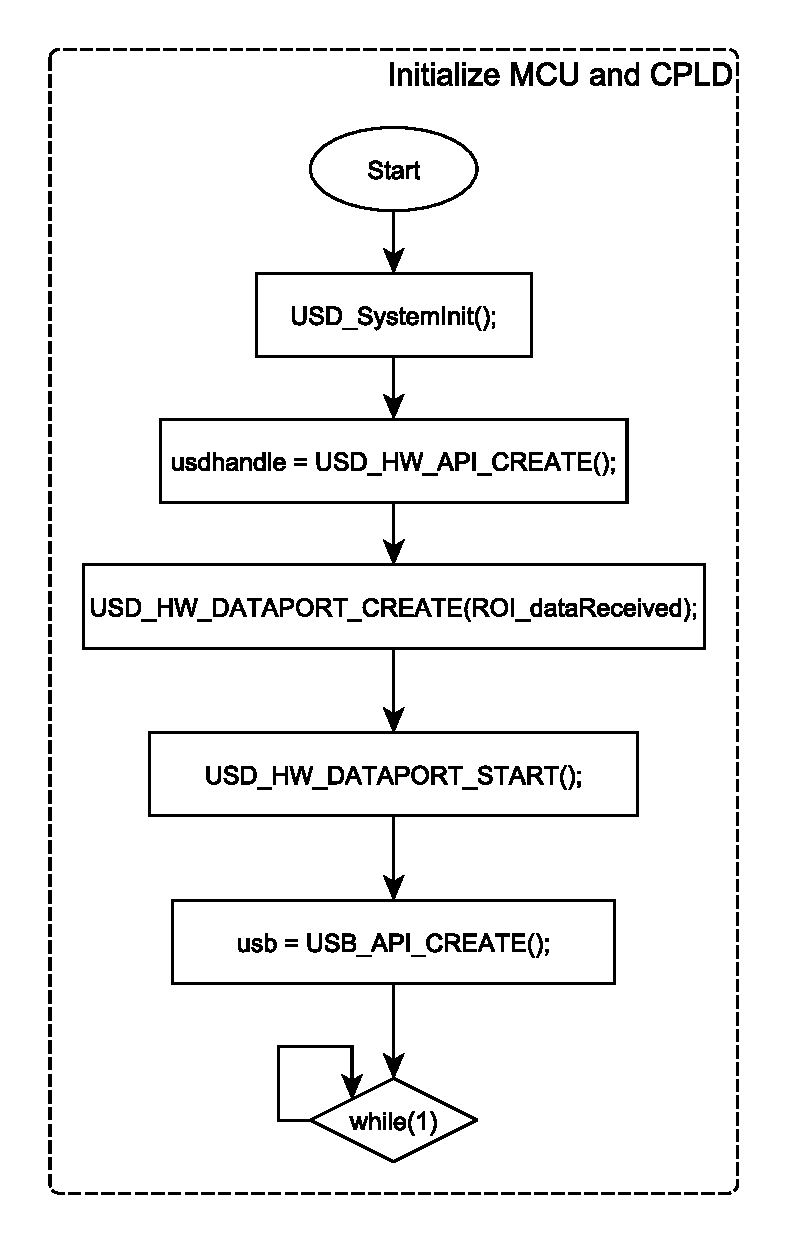
\includegraphics[width=1\textwidth, trim=0mm 0mm 0mm 0mm, clip=true]{images/software/init.eps}%28 links
	    		\caption{Ablaufdiagramm der Systeminitialisierung}
	    		\label{fig:ablaufInit}
        \end{subfigure}
        ~ %add desired spacing between images, e. g. ~, \quad, \qquad, \hfill etc.
          %(or a blank line to force the subfigure onto a new line)
        \begin{subfigure}[t]{0.52\textwidth}
        	 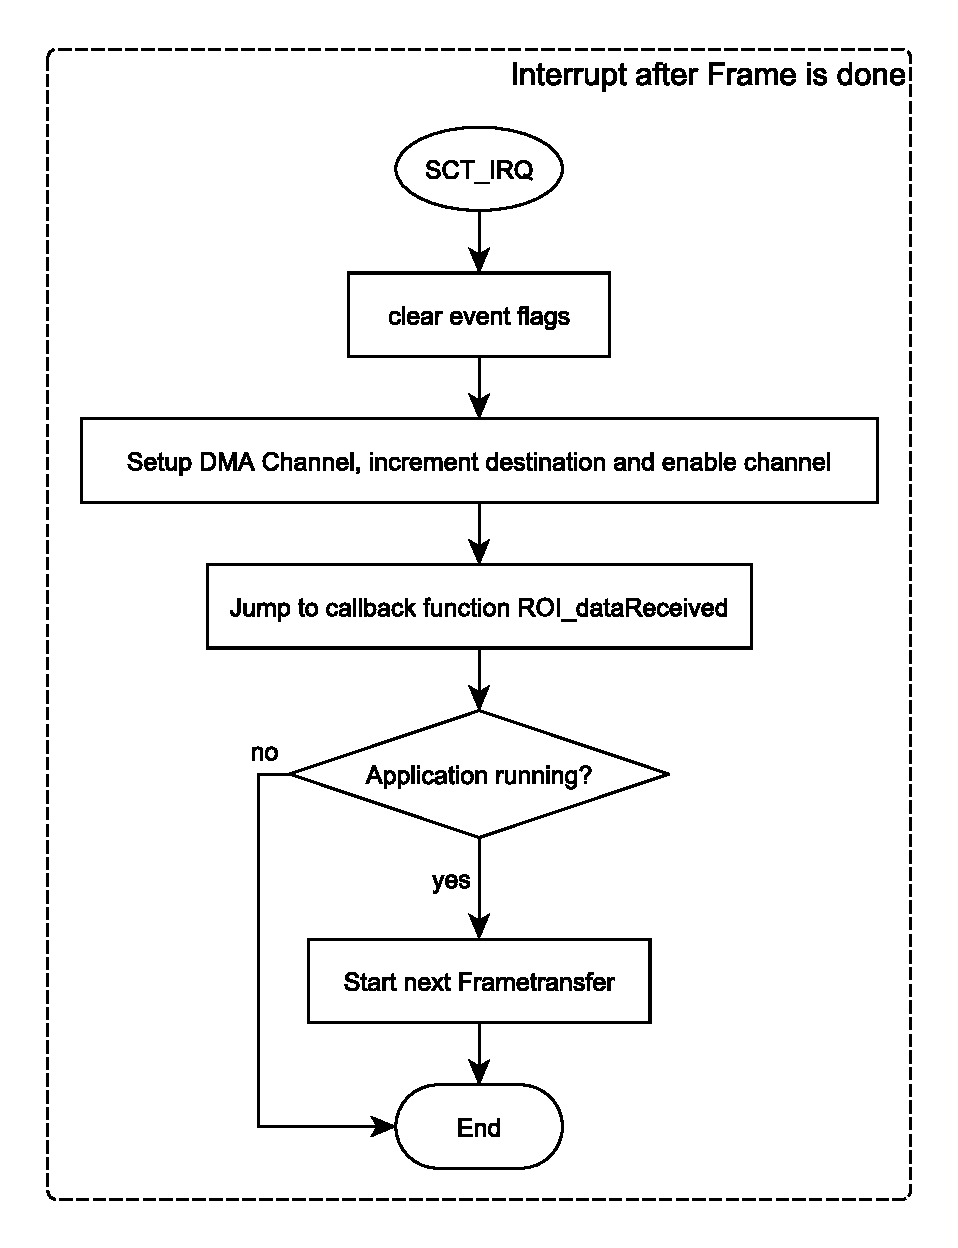
\includegraphics[width=1\textwidth, trim=0mm 0mm 0mm 0mm, clip=true]{images/software/sct_irq.eps}%28 links
	    		\caption{Ablaufdiagramm bei einen SCT Interrupt}
	    		\label{fig:Ablaufsct_interrupt}
        \end{subfigure}
        ~
        \begin{subfigure}[b]{0.65\textwidth}
        	 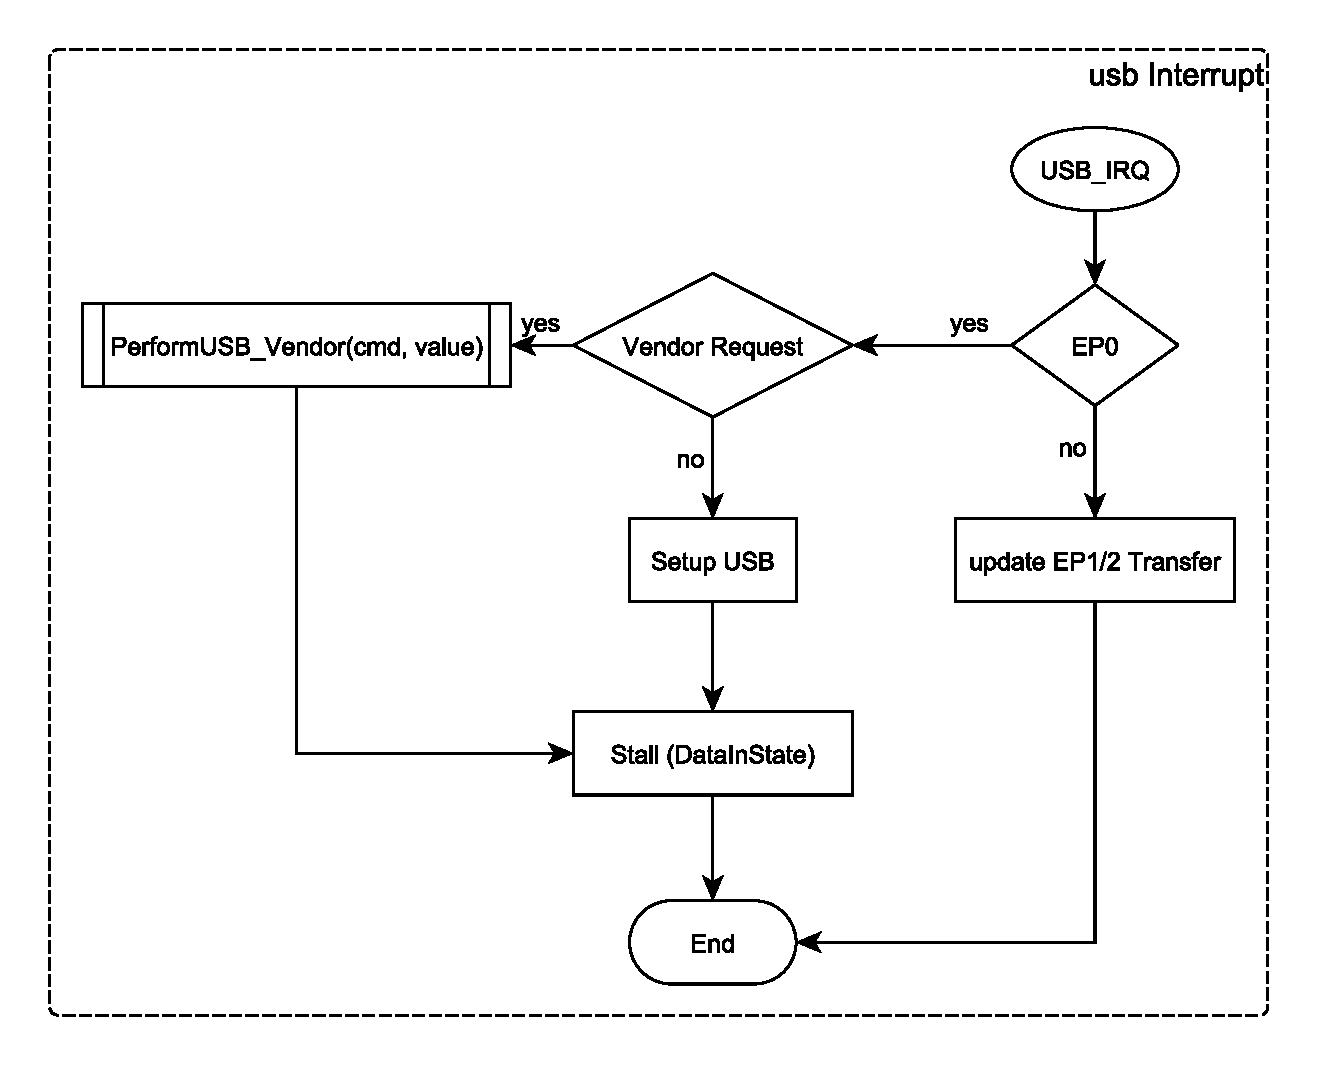
\includegraphics[width=1\textwidth, trim=0mm 0mm 0mm 0mm, clip=true]{images/software/usb_irq.eps}%28 links
	    		\caption{Ablaufdiagramm bei einen USB Interrupt}
	    		\label{fig:Ablaufusb_interrupt}
        \end{subfigure}        
\end{figure}
\clearpage
\begin{figure}[h!]
\ContinuedFloat
        \centering
        \begin{subfigure}[b]{0.89\textwidth}
        	 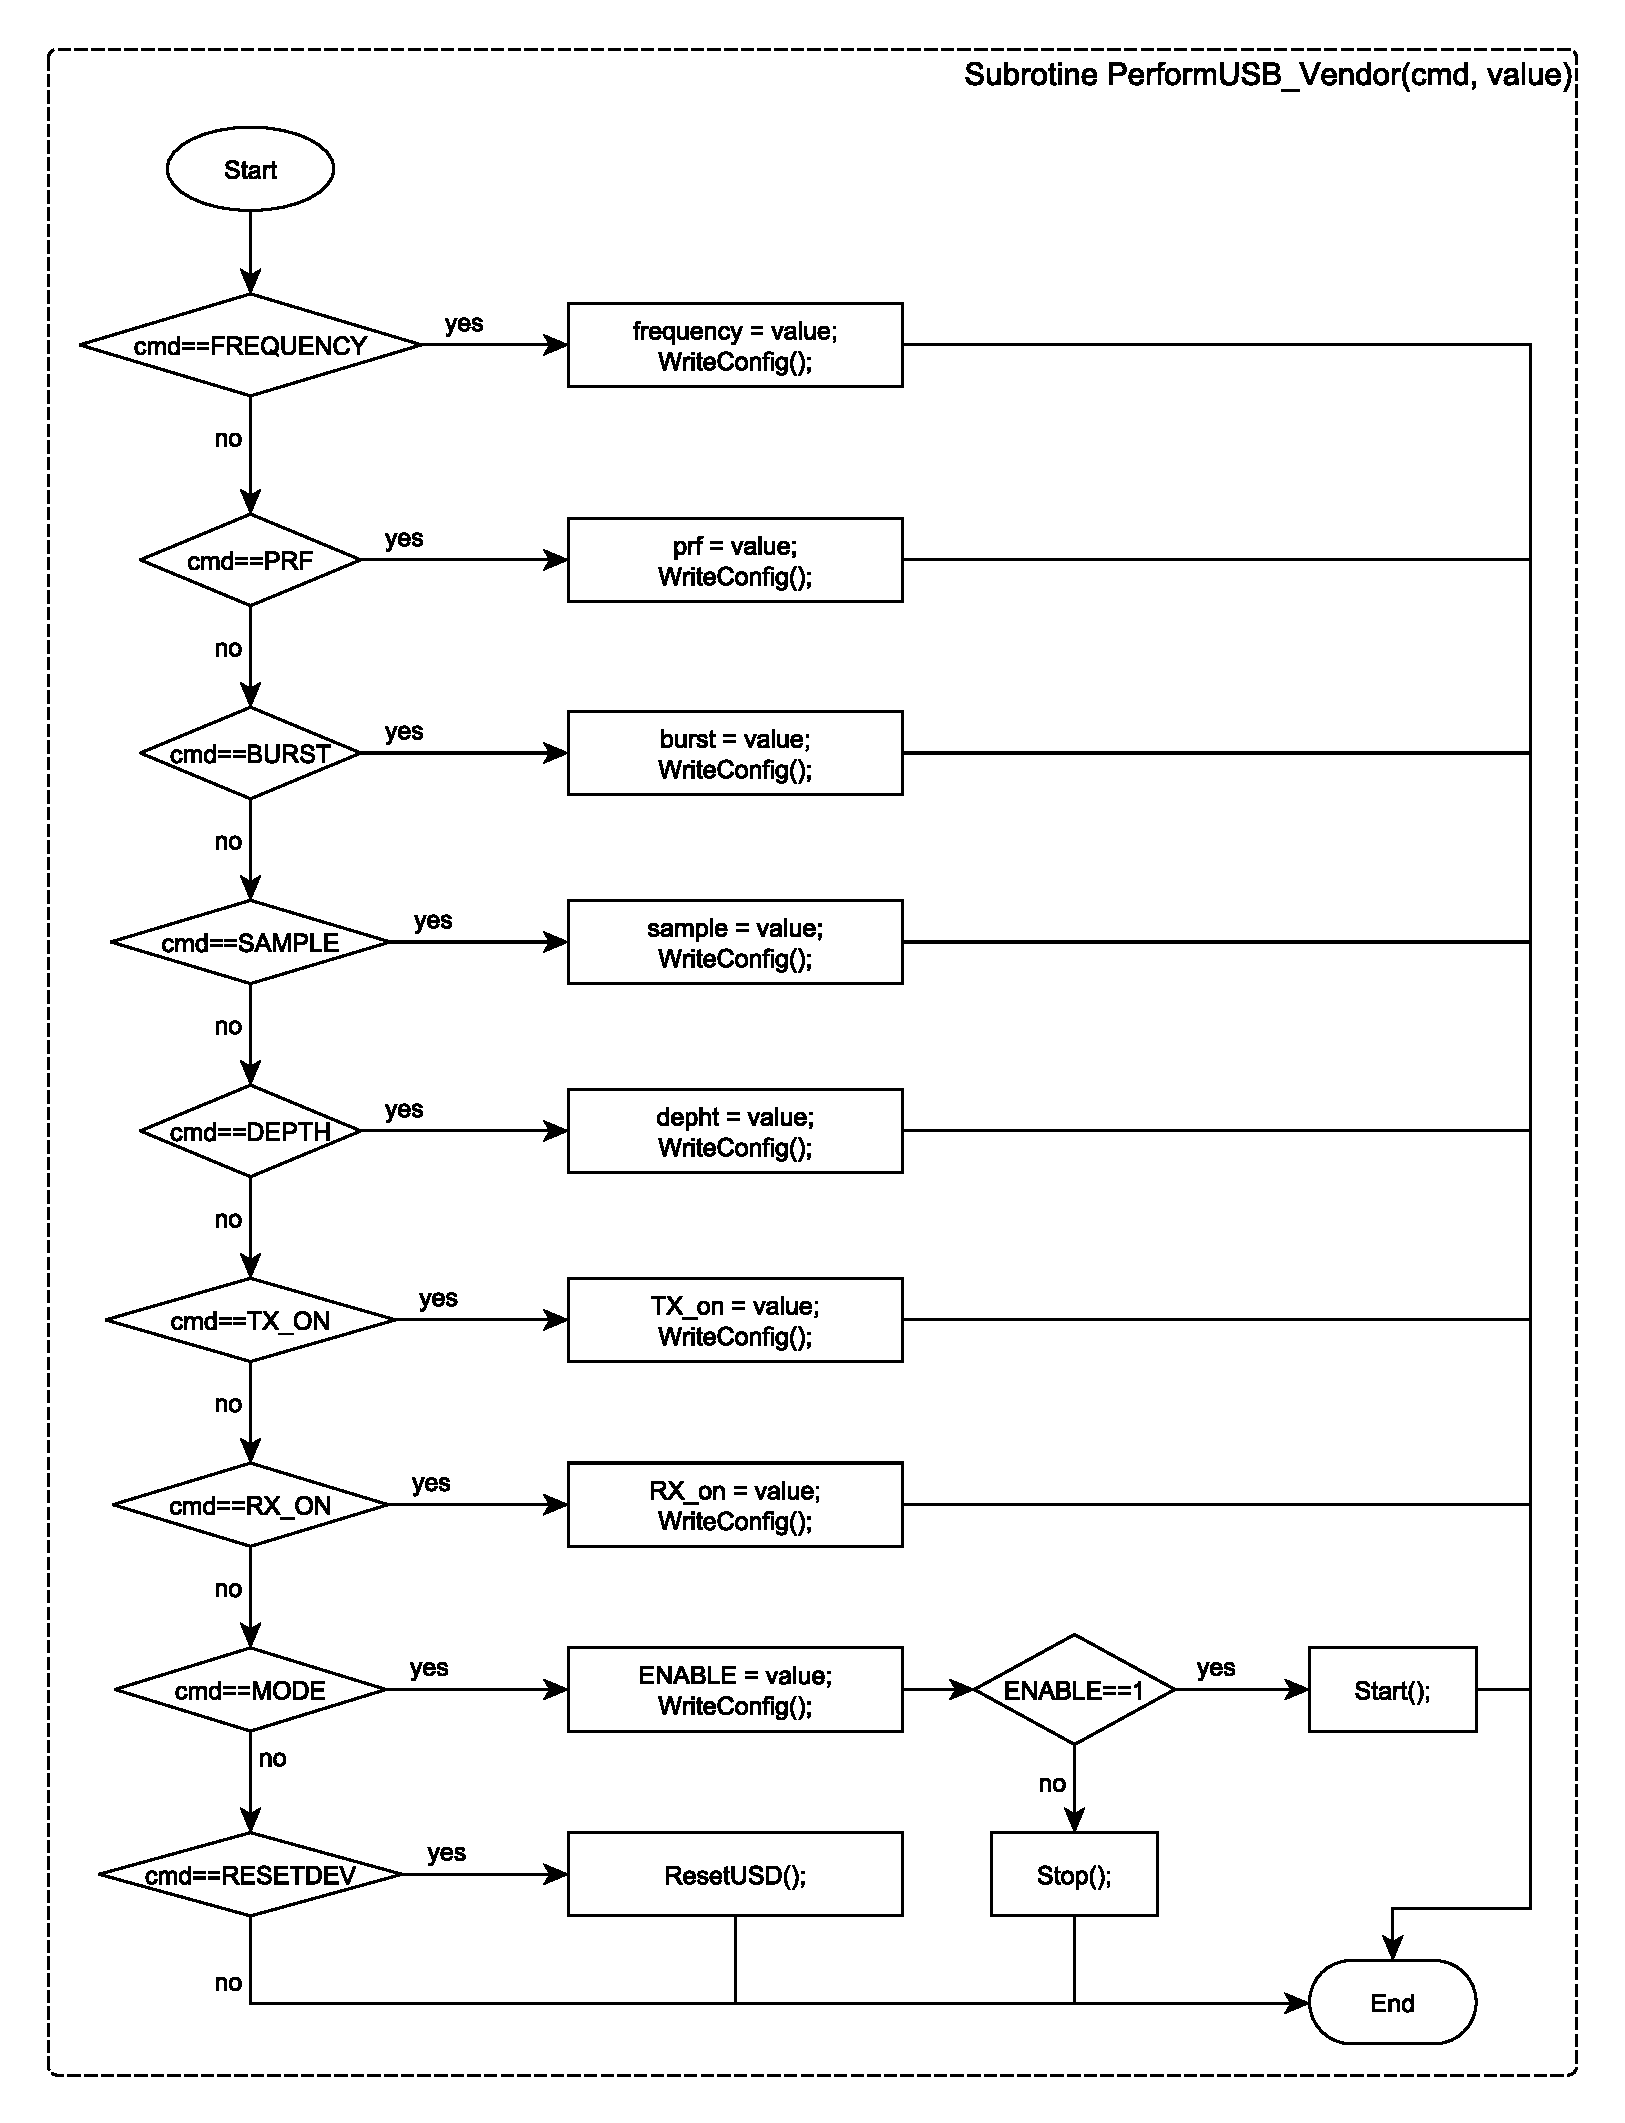
\includegraphics[width=1\textwidth, trim=0mm 0mm 0mm 0mm, clip=true]{images/software/usb_vendor.eps}%28 links
	    		\caption{Ablaufdiagramm bei einen USB Vendor Request über Endpoint 0}
	    		\label{fig:Ablaufusb_vendor}
        \end{subfigure}
        %
        \caption{Ablaufdiagramme des Systems}\label{fig:ablaufdiagramme}
\end{figure}
Durch den Aufruf des Befehls \texttt{WriteConfig()} nach der Zuweisung eines Parameters wird das \ac{cpld} mit den neuen Einstellung parametriert, wodurch das System auf Reaktionen des Benutzers sofort reagieren kann. Diese Funktionalität erlaubt eine Änderung der Messung OnTheFly.
\clearpage
\section{Visualisierung}
Da die Daten auf einen \ac{pc} visualisiert werden und nach \nameref{sec:userreq} mit verschiedenen Betriebssystemen funktionieren soll kam nur die Sprache C/C++ in Frage. Zudem wird eine GUI benötigt, welche dem Benutzer die Daten visualisiert und Eingabemöglichkeiten über Schaltflächen bietet. Aus diesen Gründen wurde sich für die \ac{api} QT entschieden, da diese \ac{api} durch die Sprache C++ sehr schnell ist und Erweiterungen für das Plotten von Echtzeitgraphiken vorhanden sind.\\
In diesem Kapitel wird die Anbindung des Systems über die \ac{usb} 2.0 Schnittstelle, das Benutzerinterface sowie die Aufbereitung der Daten für die Visualisierung beschrieben.
\subsection{Bibliotheken}
Für die Visualisierung der M-Mode und Spektrum Graphen wurde sich für das Widget QCustomPlot\cite{QCustomPlot} entschieden, da es eine hohe Performance für die Echtzeit Visualisierungen durch die Sprache C++ besitzt und leicht zu implementieren ist.  Um ein Spektrum einer Tiefe zu visualisieren müssen die Daten durch eine komplexe \ac{fft} in den Frequenzbereich gewandelt werden. Dafür wurde sich für die openSource Bibliothek kiss\_fft\cite{kissfft} entschieden, da diese durch wenige Zeilen code initialisiert und ausgeführt werden kann.\\
Um mit dem Messsystem zu kommunizieren und die Daten zu erhalten wurde die Abstrahierung der \ac{usb} Kommunikation durch die Bibliothek libusb\cite{libusb} verwendet. Da diese jedoch recht Komplex ist wurde eine \ac{api} erstellt, welche den Datentransfer der unterschiedlichen Endpoints, die Erkennung eines \ac{usb} Geräts und die grundlegenden Funktionalitäten eines Geräts abstrahiert. Somit muss für die Applikation nur eine Vererbung der Klasse usbDevice durchgeführt werden und die Erkennung erfolgt ohne weitere Implementierungen. Dies reduziert die Komplexität der Anwendung, da durch wenige Zeilen Befehle gesendet und Daten asynchron Empfangen werden können.
\subsection{\ac{gui}-Beschreibung}
\begin{figure}[h!]
	\centering
	\includegraphics[width=1\textwidth]{images/software/Programm}%28 links
	\caption[QT Programm mit M-Mode und Spektrogramm]{QT Programm mit M-Mode und Spektrogramm\cite{mmode}}
	\label{fig:programm}
\end{figure}
\autoref{fig:programm} beschreibt das grundlegende Aussehen der Anwendung. Dabei soll die Software intuitiv benutzbar sein und ohne große Erklärungen von Studenten und Endanwendern bedienbar sein. Die Menüleiste ist Schlicht gehalten, indem diese Konfigurationen zu Verfügung stellt sowie Konfigurationen Laden und Speichern kann. Zudem wurde der Reiter Ultrasonic Doppler hinzugefügt, welcher die selben Optionen wie das Docking Panel \textit{Settings} bereitstellt. Wenn der Nutzer nähere Informationen zu dem Programm benötigt, kann dieser unter den Reiter \textit{Help} das About Menü Aufrufen und über einen Link zu der Dokumentation gehen. Hierbei ist zu erwähnen, dass die Zieladresse und der Inhalt der Dokumentation noch nicht definiert ist, jedoch Vorgesehen wurde.\\
Der Bildschirm wurde in drei Bereiche gegliedert. Der erste Bereich ist die Anzeige der Doppler Daten als M-Mode sowie ein Schieberegler (in \autoref{fig:programm} nicht zusehen), wodurch die Tiefenbereiche näher betrachtet werden können. Somit kann der Nutzer die für Ihn interessanteste Tiefe auswählen, welche im darunter liegenden zweiten Bereich durch eine Komplexe \ac{fft} näher visualisiert wird. Damit die ersten zwei Bereiche auch Daten von der Instrumentierung erhalten, muss diese parametriert werden. Dies geschieht über den dritten Bereich des Docking Panels \textit{Settings}. In diesen kann die \ac{prf}, die Starttiefe der Messung sowie die Länge der \ac{roi} eingestellt werden. Aktuell kann die Trägerfrequenz noch über das Menü eingestellt werden, welches später durch die automatische Erkennung der Transducer entfällt. Dies wurde jedoch für den aktuellen Stand der Entwicklung entfernt, da Messungen bei unterschiedlichen Frequenzen durchgeführt werden mussten. Zudem kann der Nutzer den Transmitter, Receiver, sowie die Instrumentierung de- und aktivieren und das Gerät in einen definierten Zustand bringen.\\
Eine Implementierung für die Erzeugung von Tönen für den Linken und Rechten Hörkanal ist vorgesehen, um den Nutzer nicht nur visuell sondern auch akustisch das Signal mit möglichen Embolien zu verdeutlichen, \ac{bzw} diesen auf eine mögliche Embolie aufmerksam zu machen.
\subsection{Programmablauf}
\newpage